\section{Fractional-Calculus Stochastic Models for Marine Motion:
Potential Advantages and Research Directions}
\label{sec:fractional}

The following is an exploratory scientific component, not an
implementation or hardware result. The relevant question is whether a
noninteger-order stochastic model gives a better \emph{representation of
vessel displacement under IMU observation}, at an acceptable state and
compute budget, than the rational models above. A lower spectral fitting
error alone cannot answer that question. The independent-axis CARMA
experiments in \texttt{docs/carma-three-axis.md} supply an important
complete-INS comparison, but not evidence for a fractional estimator.

\subsection{Physical Memory, Stochastic Memory, and the Target Spectrum}
\label{sec:frac-motivation}
Irregular wave motion combines resonances, a broad frequency band, two or
more characteristic wave periods, and sea states evolving over much longer
times. Fluid forces on an accelerating hull also depend on its prior motion.
For small-amplitude, linearized, zero-forward-speed vessel dynamics, the
Cummins equation has the schematic multiaxis form
\begin{equation}
\begin{aligned}
(M+A_\infty)\ddot{\bm p}(t)+C\bm p(t)
&+D_v\dot{\bm p}(t)\\
{}+\int_0^t K(t-\tau)\dot{\bm p}(\tau)\,d\tau
&=\bm F_{\rm exc}(t).
\end{aligned}
\label{eq:frac-cummins}
\end{equation}
The matrix retardation kernel \(K(t)\) represents \emph{physical radiation
memory}, while wave excitation is determined by the incident directional
sea \cite{cummins62,perezfossen08,kaasen20}. A statistical fractional kernel
in a displacement prior is instead a \emph{phenomenological} description
unless its order and response have been identified against hydrodynamic
data. A nonlocal fractional kernel is not intrinsically more physical
than a stable, passive rational approximation to a measured radiation
impedance. Rational radiation-memory models with shared multiaxis poles
already exist \cite{perezfossen08,kaasen20}.

Let \(S_\eta(\omega,\beta)\) be the incident elevation directional
spectrum, and let \(R_i(\omega,\beta)\) be the complex response amplitude
operator (RAO) for vessel axis \(i\). Under the linear, stationary
approximation, the vessel cross-spectrum is
\begin{equation}
S_{p_i p_j}(\omega)=\int
 R_i(\omega,\beta) S_\eta(\omega,\beta)
 R_j(\omega,\beta)^*\,d\beta.
\label{eq:frac-rao}
\end{equation}
Encounter-frequency transformations, heading, speed, directional spread,
and hull-dependent RAOs can shift peaks and change high-frequency slopes.
Accordingly, Pierson--Moskowitz (PM) and JONSWAP are \emph{incident-wave}
references \cite{pierson64,hasselmann73}, not universal displacement priors.
This distinction is decisive: matching an idealized incident tail more
closely need not yield a better heave, surge, or sway estimate.

There are also different kinds of temporal memory. Statistical
long-range dependence normally refers to slowly decaying covariance or a
low-frequency spectral singularity. A fractional operator can have a
nonlocal impulse response while its covariance remains short-range, e.g.,
because a stable oscillator exponentially tempers the memory. Oscillation,
memory, and accurate low-frequency suppression are separate properties.

\subsection{Fractional Brownian Motion, Fractional OU, and CARFIMA}
\label{sec:frac-processes}
\subsubsection{Fractional Brownian motion and Gaussian noise}
Fractional Brownian motion \(B_H(t)\), \(0<H<1\), is the centered Gaussian
process with covariance \cite{mandelbrot68}
\begin{equation}
\E B_H(t)B_H(s)=\tfrac12\bigl(
 |t|^{2H}+|s|^{2H}-|t-s|^{2H}\bigr).
\label{eq:frac-fbm}
\end{equation}
Its increments (fractional Gaussian noise, fGn, after sampling) are
stationary, whereas \(B_H\) itself is not: its variance grows as
\(|t|^{2H}\). For the generalized continuous-time derivative of \(B_H\),
the two-sided spectrum scales as
\(S_{\dot B_H}(\omega)\propto|\omega|^{1-2H}\).
Values \(H>1/2\) imply persistent increments and low-frequency
enhancement; \(H<1/2\) imply antipersistence and suppression. Directly
using fBm as heave displacement would import nonstationary variance and
potential integration drift into a filter already sensitive to acceleration
bias. fGn can model a stochastic \emph{excitation}, but stronger
correlations are not automatically informative: low-frequency excitation
can become observationally confounded with residual accelerometer bias.

\subsubsection{Fractional Ornstein--Uhlenbeck processes}
One stationary construction integrates fBm against an exponential kernel:
\begin{equation}
X_H(t)=\sigma_H\int_{-\infty}^{t}
 e^{-\lambda(t-u)}\,dB_H(u),\quad\lambda>0.
\label{eq:frac-fou}
\end{equation}
For the appropriate generalized stochastic integral, its spectrum is
\begin{equation}
S_{X_H}(\omega)\propto
\frac{|\omega|^{1-2H}}{\lambda^2+\omega^2}.
\label{eq:frac-fou-psd}
\end{equation}
This is \emph{one} fractional OU definition; alternative constructions
and transformations need not have identical covariance
\cite{cheridito03}. For \(H>1/2\) it permits slow persistence, and
for \(H<1/2\) it removes low-frequency power, but a single relaxation
factor does not ordinarily create a pronounced nonzero-frequency wave
resonance. It may be more suitable for slowly changing wave-envelope,
amplitude, or spectral parameters. Making those parameters stochastic
also makes the conditional estimator time varying or nonlinear and
requires explicit parameter/state covariance handling.

\subsubsection{CARFIMA and fractionally integrated CARMA}
Tsai's CARFIMA construction uses fBm-driven continuous-time
autoregressive/moving-average dynamics and has, under its stationarity
and integrability hypotheses, the spectral form \cite{tsai09}
\begin{equation}
S_{\rm CF}(\omega)=c_H\sigma^2|\omega|^{1-2H}
 \frac{|b(i\omega)|^2}{|a(i\omega)|^2},\quad c_H>0.
\label{eq:frac-carfima}
\end{equation}
For \(H=1/2\), the fractional forcing reduces to white forcing.
Writing \(d=H-1/2\) exposes the idealized fractional-integration
factor \(|\omega|^{-2d}\). The \emph{combined} transfer determines the
low-frequency response: multiplying a DC-zero CARMA(4,1) spectrum by
this factor changes \(S_p\sim|\omega|^2\) to
\(S_p\sim|\omega|^{2-2d}\), which still tends to zero for the
usual \(-1/2<d<1/2\). By contrast, applying it to the actual
experimental CARMA(5,2) numerator with a nonzero DC term produces
\(S_p\sim|\omega|^{-2d}\); positive \(d\) then enhances weakly
observed near-DC motion. A formal CARMA(4,1) relative-degree-three
tail becomes \(|\omega|^{-6-2d}\) at high frequency; its ideal
acceleration remains finite for \(d>-1/2\), subject to the complete
stationary construction. Such non-tempered integration brings memory
near zero frequency, where real vessel translation, gravity projection,
and bias can be hard to distinguish. The operator cannot be judged by
the fractional parameter alone.

\subsection{Primary Candidate: A Fractional-Powered Oscillator}
\label{sec:frac-primary}
Let \(f_0=\omega_0/(2\pi)>0\) and \(\zeta>0\), with
\(L(s)=s^2+2\zeta\omega_0s+\omega_0^2\). Define the \emph{causal
stationary Gaussian filtered-noise process} by
\begin{equation}
H_\nu(s)=\frac{\sigma s}{L(s)^\nu},\qquad
p(t)=(h_\nu*\xi)(t),
\label{eq:frac-hnu}
\end{equation}
where \(\xi=dW_t/dt\) is generalized white noise with
\(\E\xi(t)\xi(t')=\delta(t-t')\), and the fractional power is
the causal analytic branch obtained by taking powers of the two stable
linear pole factors. Assume \(\nu>3/4\) and a stationary infinite-past
initialization. With \(p\) in metres and time in seconds,
\([\sigma]=\mathrm{m\,s}^{3/2-2\nu}\).

We use the \emph{two-sided angular-frequency} convention
\begin{equation}
\E p^2=\frac{1}{2\pi}\int_{-\infty}^{\infty}
 S_p^{(\omega)}(\omega)\,d\omega,\qquad
 S_p^{(f)}(f)=2S_p^{(\omega)}(2\pi f),\ f>0.
\label{eq:frac-convention}
\end{equation}
Independently substituting \(s=i\omega\) and using the flat unit
angular-spectrum of \(\xi\) gives
\begin{equation}
\boxed{S_p^{(\omega)}(\omega)=
q\frac{\omega^2}{\bigl[(\omega_0^2-\omega^2)^2+
(2\zeta\omega_0\omega)^2\bigr]^\nu}},\ q=\sigma^2.
\label{eq:frac-psd}
\end{equation}
Thus \(q\) has units \(\mathrm{m^2\,s}^{3-4\nu}\), and the
one-sided \(S_p^{(f)}\) has units \(\mathrm{m^2/Hz}\). This
derivation uses the modulus of the \emph{fractional power}:
\(|L(i\omega)^\nu|^2=|L(i\omega)|^{2\nu}\); it does not
incorrectly exponentiate the numerator or insert an extra
\(2\pi\) in the angular-frequency spectrum.

For \(\zeta>0\), the roots of \(L\) lie strictly in the left
half-plane. The specified branch of \(L^{-\nu}\) is analytic for
\(\Re s\ge0\); its causal kernel is a convolution of exponentially
tempered fractional kernels. The derivative in the numerator does not
make the output stationary unless the resulting impulse response is
square integrable. At high frequency
\(H_\nu(i\omega)=O(|\omega|^{1-2\nu})\), so that is true
exactly when \(\nu>3/4\) for this nondegenerate model.
This is mean-square stationary stability, not a claim of deterministic
global boundedness or nonlinear filter stability.

Direct expansion gives
\begin{align}
S_p^{(\omega)}(\omega)&\sim
q\omega_0^{-4\nu}\omega^2,&\omega&\to0,\label{eq:frac-low}\\
S_p^{(\omega)}(\omega)&\sim
q|\omega|^{2-4\nu},&|\omega|&\to\infty.
\label{eq:frac-high}
\end{align}
For the \(k\)-th mean-square derivative, the high-frequency variance
integrand is \(\omega^{2k}S_p\sim|\omega|^{2k+2-4\nu}\).
Its integral converges if and only if
\begin{equation}
\boxed{\nu>\frac{2k+3}{4}:\quad
\begin{cases}
k=0:\ \nu>3/4,\\
k=1:\ \nu>5/4,\\
k=2:\ \nu>7/4.
\end{cases}}
\label{eq:frac-moments}
\end{equation}
Equality gives a logarithmically divergent moment. In particular,
the \(\nu=1.80\)--\(2.00\) illustrations permit finite-variance
ideal acceleration; adding finite measurement bandwidth changes the
practical regularity requirement but not this continuous-time result.
Finite moments do \emph{not} imply that a nondegenerate stationary
Gaussian realization is almost surely bounded uniformly over an
unlimited time horizon.

The single factor \(s\) also has a useful low-frequency consequence:
\(p=\dot X\) in mean square for
\(H_X(s)=\sigma/L(s)^\nu\). Hence an additional time integral
\(\int_{t_0}^t p(u)du=X(t)-X(t_0)\) has uniformly finite
variance for the admissible \(\nu>3/4\); there is no \emph{variance}
random walk from this idealized DC-zero prior. This does not enforce a
bounded sample path, protect against a biased accelerometer, or extend
to integrating a nonzero-DC spectral component. The integral's separate
stationary primitive needs only \(\nu>1/4\), but the proposed
\(p\) needs the stronger condition above.

Writing \(r=(\omega/\omega_0)^2\) and \(a=4\zeta^2-2\), the
nonzero-frequency peak satisfies
\begin{equation}
(1-2\nu)r^2+(1-\nu)ar+1=0.
\label{eq:frac-peak}
\end{equation}
For \(\nu>1/2\), this quadratic has exactly one positive root:
this \emph{single} fractional oscillator cannot have two separated
spectral maxima. Both \(\nu\) and \(\zeta\) change its peak, bandwidth,
and shoulders; they can also be partially confounded by spectral fitting.
Although \(\nu=1.75\) would give a \(|\omega|^{-5}\) displacement
tail close to the incident PM/JONSWAP exponent, it fails the
finite-variance ideal acceleration test at equality. At \(\nu=1.85\),
the displacement and acceleration tails are \(|\omega|^{-5.4}\)
and \(|\omega|^{-1.4}\), respectively; at \(\nu=2\) they are
\(|\omega|^{-6}\) and \(|\omega|^{-2}\).

At the integer limit,
\begin{equation}
H_2(s)=\frac{\sigma s}{L(s)L(s)},
\label{eq:frac-integer}
\end{equation}
which is a \emph{constrained} CARMA(4,1) realization with two identical
oscillator factors, not an arbitrary CARMA(4,1) with independently
adjustable poles. For noninteger \(\nu\), the transfer has branch
singularities and no exact fixed finite-dimensional rational Markov
realization. Its memory is exponentially tempered by the stable
oscillator poles, so noninteger order here does \emph{not} imply the
long-range dependence of fGn.

\subsection{Fractional Damping and Tempered CARMA Shaping}
\label{sec:frac-alternatives}
Fractional damping changes the equation of motion rather than raising
the complete stable oscillator to a fractional power:
\begin{equation}
\ddot p+cD^\alpha p+\omega_0^2p=\sigma\xi,
\qquad 0<\alpha<1.
\label{eq:frac-damping}
\end{equation}
For a stationary infinite-past construction, a suitable
Riemann--Liouville/Weyl derivative has Fourier multiplier
\((i\omega)^\alpha\); a Caputo initial-value formulation requires
initial-condition terms and should not be substituted without care.
Here \(c>0\) has units \(\mathrm{s}^{\alpha-2}\).
The formal stationary transfer is
\(H_\alpha(s)=\sigma/(s^2+cs^\alpha+\omega_0^2)\).
It has \emph{nonzero} zero-frequency displacement power; with raw white
forcing its high-frequency displacement tail is
\(|\omega|^{-4}\), so the ideal acceleration variance diverges.
If the kernel is causal and stable, an optional shaped candidate is
\begin{equation}
H_{\alpha,\rm sh}(s)=
\frac{\sigma s}{(s+\lambda)^2
(s^2+cs^\alpha+\omega_0^2)},\quad \lambda>0,
\label{eq:frac-damped-shaped}
\end{equation}
with zero-frequency suppression and a \(|\omega|^{-6}\)
high-frequency displacement tail. These are properties of the
\emph{shaped transfer}, not the unmodified fractional damping law;
passivity, pole/branch stability, conditioning, and physical validity
must still be checked. Fractional Langevin literature
\cite{lutz01,drozdov07} motivates this family, but neither article
validates this particular IMU prior.
Recent numerical work on fractional hydrodynamic damping in nonlinear
ship rolling \cite{mitseas26} further motivates controlled study;
it is not evidence about heave reconstruction from an IMU.

A lower-risk option is to retain the fitted CARMA(4,1) core while
adding a \emph{tempered} fractional factor,
\begin{equation}
H_T(s)=H_{4,1}(s)
 \left(\frac{s+\lambda_z}{s+\lambda_p}\right)^\delta,
\quad \lambda_z,\lambda_p>0.
\label{eq:frac-tempered}
\end{equation}
Its analytic stable branch preserves the CARMA DC zero and the
\(|\omega|^{-6}\) far-tail exponent, because the new factor tends
to a finite nonzero constant at zero and to unity at infinity.
The pole/zero ratio reshapes an intermediate band; its gain and
phase still need to be fitted, and a noninteger \(\delta\) introduces
a memory kernel and additional approximation states. This
\emph{fractionally shaped CARMA} is not the same as Tsai's
non-tempered CARFIMA process. Whether it improves parameter
identifiability is an empirical question.

\subsection{Reproducible Spectral and Motion Illustrations}
\label{sec:frac-figures}
Figures~\ref{fig:frac-spectra}--\ref{fig:frac-highpass-refit} are generated
by the checked-in Python script in this document's directory.
That script also saves a JSON record of every fit, parameter, and
numerical configuration. All spectra use the one-sided convention
(\ref{eq:frac-convention}). Figure~\ref{fig:frac-spectra}
tests a deliberately limited proposition: can the single fractional
oscillator represent an \emph{incident} JONSWAP shape when its
\(f_0,\zeta\) are numerically fitted for fixed \(\nu\)?
It does not represent a hull-response identification.

\begin{figure*}[t]
\centering
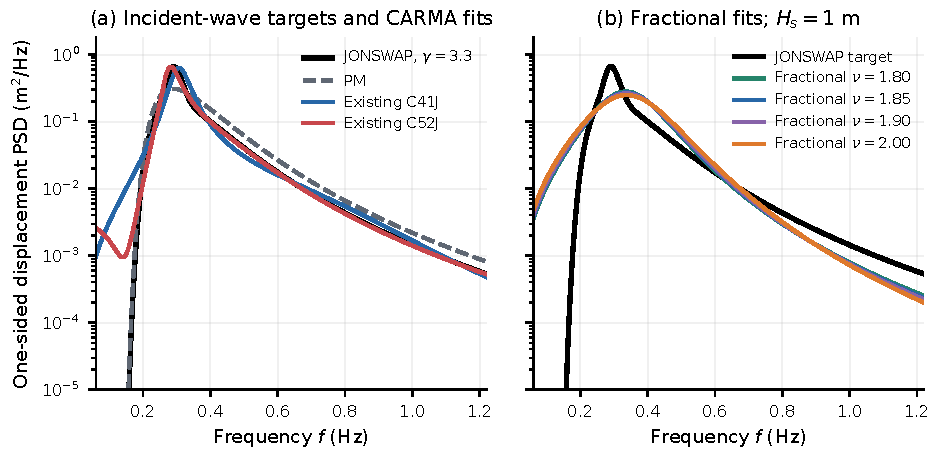
\includegraphics[width=.99\textwidth]{fractional-fig-1-spectra.pdf}
\caption{Reproducible \emph{incident-elevation} spectra, not vessel heave:
PM and JONSWAP (\(\gamma=3.3\), \(f_p=0.29\) Hz,
\(H_s=1.0\) m); existing documented JONSWAP-calibrated CARMA(4,1)
(C41J) and CARMA(5,2) (C52J) parameters; and separately optimized
fractional oscillators \(\nu=1.80,1.85,1.90,2.00\).
All curves have the same integrated displacement variance
\((H_s/4)^2\) on the 0.008--12 Hz quadrature band.
Fractional \(f_0,\zeta\) minimize weighted log-PSD residual over
0.18--1.15 Hz; the documented CARMA parameters are not refitted.
The idealized incidence comparison does not include a vessel RAO.}
\label{fig:frac-spectra}
\end{figure*}

Define the fitted log-spectral score over selected frequencies \(f_i\) by
\begin{equation}
E_{\rm dB}^2=
\frac{\sum_i w_i
 [10\log_{10}(S_{\rm model}(f_i)/S_{\rm target}(f_i))]^2}
 {\sum_i w_i},
\label{eq:frac-fit-objective}
\end{equation}
with
\(w_i=0.2+0.8[S_{\rm target}(f_i)/\max S_{\rm target}]^{0.3}\).
The model variance is fixed to the target quadrature variance, not
shifted by eye to align maxima. On this single incident JONSWAP
example the documented C41J/C52J shapes have \(E_{\rm dB}=1.82/0.87\)
dB. Refitted fractional models at \(\nu=1.80/1.85/1.90/2.00\)
have errors \(3.17/3.24/3.30/3.42\) dB. These numbers reflect
the selected band and family, not a general theorem ranking CARMA
above fractional dynamics. In particular, the fractional operator's
closer asymptotic tail does not guarantee a better fit around a
narrow peak and its shoulders.

\subsubsection{A matched-objective refit with fractional high-pass shaping}
The original four fixed-order tests do not exhaust fractional
spectral modeling. In particular, their \(\omega^2\) low-frequency
suppression is too weak to mimic the rapidly suppressed low-frequency
shoulder of an \emph{incident} JONSWAP spectrum. To test whether
additional fractional shaping changes that result, introduce
\begin{equation}
H_{\nu,\eta}(s)=\frac{\sigma s}{L(s)^\nu}
  \left(\frac{s}{s+\lambda}\right)^\eta,
\quad \eta\geq0,\ \lambda>0,
\label{eq:frac-highpass}
\end{equation}
where \(L(s)=s^2+2\zeta\omega_0s+\omega_0^2\),
\(\lambda\) has units \(\mathrm{rad\,s^{-1}}\),
and the fractional factor uses the analytic branch in
\(\operatorname{Re}s>0\). Because
\(\operatorname{Re}[s/(s+\lambda)]>0\) there, that factor is
analytic and bounded for positive real \(\eta\). Combined with
the stable fractional oscillator, it defines a causal stationary
Gaussian output under the variance conditions already derived.
Its PSD, for the same white-noise intensity convention as
(\ref{eq:frac-psd}), is
\begin{equation}
S_{\nu,\eta}(\omega)=q\frac{\omega^2}{|L(i\omega)|^{2\nu}}
\left(\frac{\omega^2}{\omega^2+\lambda^2}\right)^\eta.
\label{eq:frac-highpass-psd}
\end{equation}
At low frequencies the spectrum now behaves as
\(\omega^{2+2\eta}\), whereas its high-frequency exponent
remains \(2-4\nu\). Thus the exact displacement, velocity,
and acceleration mean-square thresholds on \(\nu\) are unchanged.
This is a \emph{phenomenological high-pass prior}; the
fractional factor is not an identified Cummins radiation kernel.

To avoid comparing a newly fitted fractional model against
unchanged historical CARMA parameters, we refit CARMA(4,1),
CARMA(5,2), and the high-pass families using the identical
JONSWAP target, variance constraint, frequency grid, bounds,
and log-PSD objective (\ref{eq:frac-fit-objective}). Multiple
bounded initializations reduce sensitivity to local minima,
but do not establish a global optimum. For the new
\(\nu=1.80\) model, optimizing \(\eta,\lambda,f_0,\zeta\)
reduces the JONSWAP error from \(3.17\) to \(0.76\) dB;
the fitted \(\eta\approx4.72\) is \emph{not} a small
perturbation. Allowing \(\nu\) to vary gives \(\nu\approx1.96\),
\(\eta\approx4.17\), and only a marginal further improvement
to \(0.758\) dB. These are real numerical spectral improvements
within the more flexible transfer family, not measured estimator
improvements.

\begin{figure*}[t]
\centering
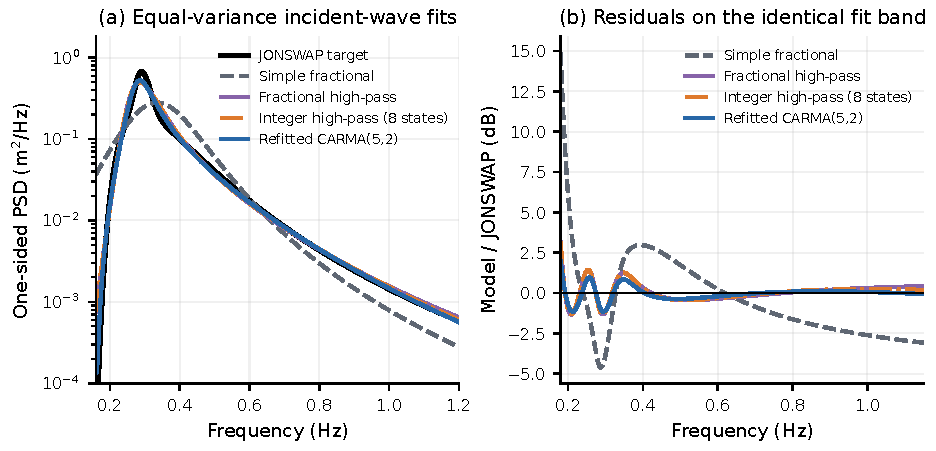
\includegraphics[width=.99\textwidth]{fractional-fig-7-highpass-refit.pdf}
\caption{\emph{Matched-objective} incident JONSWAP fitting:
original single fractional oscillator \(\nu=1.80\),
new fractional high-pass shaper at fixed \(\nu=1.80\),
integer high-pass control \(\nu=2,\eta=4\), and independently
refitted CARMA(5,2). Left: fitted one-sided spectra with
the common \((H_s/4)^2\) variance. Right: log-PSD residuals
over the same 0.18--1.15 Hz band. High-pass fractional
shaping improves the original fractional fit substantially,
but the similarly effective integer control and the better
CARMA(5,2) refit prevent attribution of a unique fractional
advantage. No hull RAO or INS measurements are included.}
\label{fig:frac-highpass-refit}
\end{figure*}

\begin{table*}[t]
\centering
\caption{Separate bounded, multi-start fits to incident JONSWAP
(\(\gamma=3.3\)) and PM (\(\gamma=1\)), both with
\(f_p=0.29\) Hz, \(H_s=1\) m. Lower is better. The JONSWAP
peak-band metric is normalized \(L_2\) spectral error over
0.24--0.48 Hz; the other scores use (\ref{eq:frac-fit-objective})
over 0.18--1.15 Hz. PM parameters are fitted anew, not transferred
from JONSWAP. Exact wave-state count applies only to rational
models; noninteger models need approximation.}
\label{tab:frac-fair-refit}
\footnotesize
\begin{tabular}{lrrrr}
\hline
Model & JONSWAP (dB) & Peak \(L_2\) (\%) & PM (dB) & Exact states/axis \\
\hline
CARMA(4,1), refitted & 1.61 & 16.2 & --- & 4 \\
CARMA(5,2), refitted & \textbf{0.58} & 17.5 & \textbf{0.21} & 5 \\
Single fractional, \(\nu=1.80\) & 3.17 & --- & --- & non-Markov \\
Fractional high-pass, \(\nu=1.80\) & 0.76 & 21.2 & 0.59 & non-Markov \\
Fractional high-pass, free \(\nu\) & 0.76 & 21.5 & 0.43 & non-Markov \\
Integer high-pass, \(\nu=2,\eta=4\) & 0.76 & 21.3 & 0.66 & 8 \\
\hline
\end{tabular}
\end{table*}

The more flexible fit is \emph{not} evidence that fractional
memory is essential. Indeed, the integer-order control
\begin{equation}
H_{2,4}(s)=\frac{\sigma s^5}{L(s)^2(s+\lambda)^4}
\label{eq:frac-integer-highpass}
\end{equation}
achieves \(0.759\) dB on JONSWAP, essentially indistinguishable
from the best fractional high-pass score under this metric.
It is an exact \emph{eight-state-per-axis} rational process,
versus five states for CARMA(5,2), and its XYZ use would
nominally require \(33\) total states with the same nine
non-wave INS states. A fractional high-pass requires a
separate finite-band rational approximation and may require
more states; the necessary order has \emph{not} been measured.
Allowing CARMA(5,2) to refit the same objective obtains
\(0.577\) dB, and its PM refit obtains \(0.207\) dB versus
\(0.431\) dB for the free-fractional high-pass. Furthermore,
the fractionally shaped JONSWAP fit has about \(21\%\)
peak-band relative \(L_2\) error versus \(17.5\%\) for the
refitted CARMA(5,2). Some CARMA refit parameters reach
the supplied optimization bounds and require physical
qualification before use. The original negative result was
\emph{family-specific}; the new positive shaping result is
\emph{not a cost-matched win}. Neither metric tests estimator
startup, bias rejection, or covariance consistency.

\begin{figure*}[t]
\centering
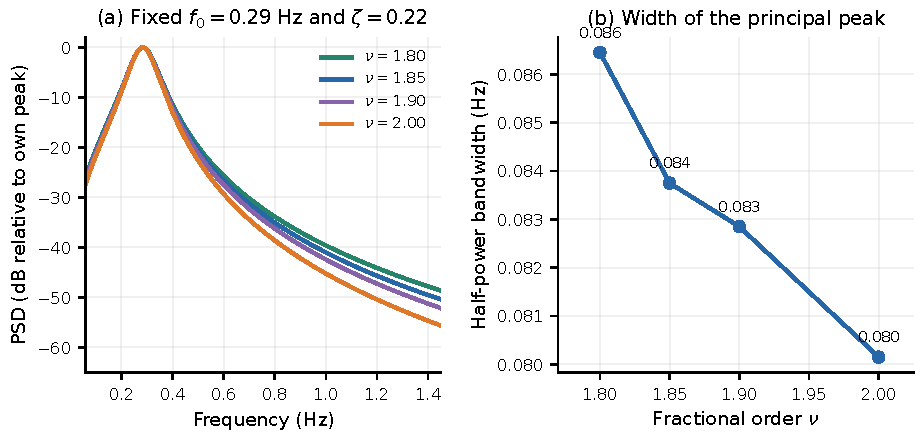
\includegraphics[width=.99\textwidth]{fractional-fig-2-order-sensitivity.pdf}
\caption{Fractional-order sensitivity for \emph{fixed}
\(f_0=0.29\) Hz, \(\zeta=0.22\).
Left: each theoretical spectrum is expressed in dB relative to
its own peak, so only shape is compared. Right: principal-peak
half-power width versus \(\nu\), computed from dense sampled spectra.
Increasing \(\nu\) changes the peak and tail simultaneously; the
bandwidth is not a free independent tuning knob.}
\label{fig:frac-sensitivity}
\end{figure*}

\begin{figure*}[t]
\centering
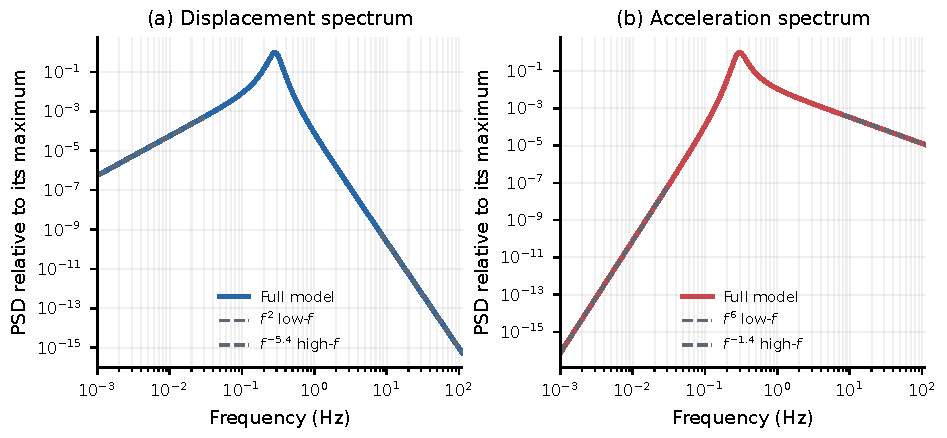
\includegraphics[width=.99\textwidth]{fractional-fig-3-asymptotic-slopes.pdf}
\caption{Log--log displacement and ideal acceleration spectral
asymptotics for \(\nu=1.85\), with each spectrum divided by its
own peak. Displacement has slopes \(+2\) at zero and \(-5.4\)
at infinity. Multiplication by \((2\pi f)^4\) gives
acceleration slopes \(+6\) and \(-1.4\).
The latter is integrable; \(\nu=1.75\) would instead give the
non-integrable limiting acceleration slope \(-1\).
Dashed segments are theoretical power-law guides.}
\label{fig:frac-slopes}
\end{figure*}

\begin{figure*}[t]
\centering
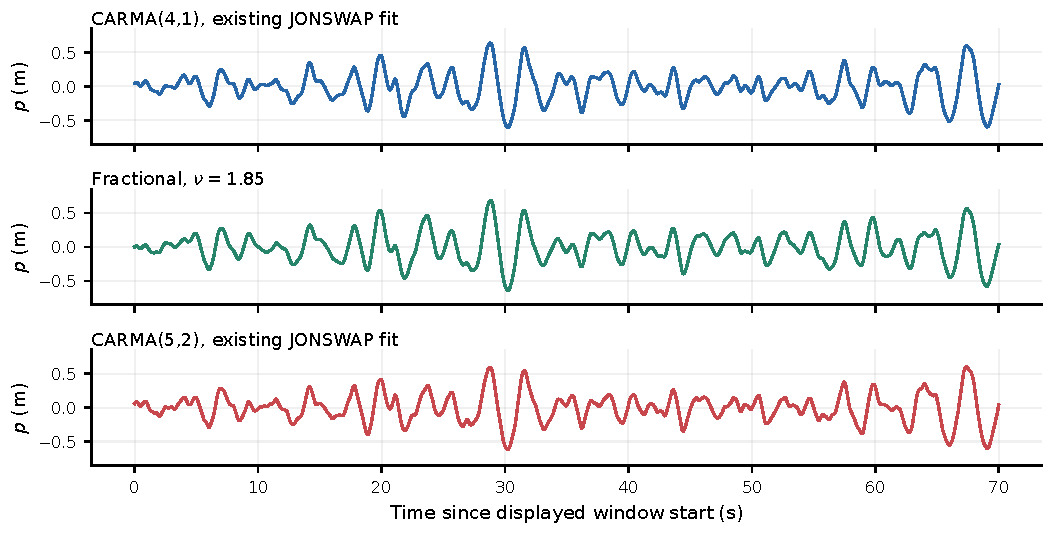
\includegraphics[width=.99\textwidth]{fractional-fig-4-realizations.pdf}
\caption{Representative stationary stochastic displacement draws,
not measured vessel motion. One common seeded Gaussian white-noise
record (seed 20261029) is FFT-filtered by the analytic CARMA(4,1),
fractional-\(\nu=1.85\), and CARMA(5,2) spectra on a 200 Hz,
240 s periodic grid; 25--95 s is displayed. All have
theoretical target variance \(0.0625\,\mathrm{m^2}\) under
the finite-grid spectral convention. FFT synthesis is a
finite-band periodic simulation, \emph{not} a fractional
finite-state Kalman approximation. Visual smoothness is not
an estimator-accuracy metric.}
\label{fig:frac-motion}
\end{figure*}

\subsection{Finite-State Approximation and Kalman Compatibility}
\label{sec:frac-kalman}
The exact noninteger transfer is not rational and, in general, its
history cannot be encoded in a fixed finite-dimensional Markov vector.
To use a conventional finite-state Kalman filter, choose a stable
rational approximation \cite{oustaloup00,gustavsen99,beylkin05}
\begin{equation}
H_\nu(s)\simeq \frac{B_M(s)}{A_M(s)}
=C_M(sI-A_M)^{-1}G_M,
\label{eq:frac-rational}
\end{equation}
over an explicit encounter/IMU frequency band. Candidates include
vector fitting with stable-pole enforcement, exponential/Prony
approximations to the impulse kernel, frequency-limited fractional
operators, and positive-real constrained fits when physical
radiation impedance is modeled. Small magnitude residual alone is
not enough: phase, time-domain transients, pole sensitivity,
minimum-phase structure, and acceleration regularity matter.

For continuous process-noise intensity \(G_MG_M\T\succeq0\),
valid discretization at the actual sample interval \(h\) is
\begin{equation}
\begin{aligned}
F(h)&=e^{A_Mh},\\
Q(h)&=\int_0^h e^{A_Mu}G_MG_M\T
 e^{A_M\T u}\,du\succeq0.
\end{aligned}
\label{eq:frac-q}
\end{equation}
Van Loan block-exponential or numerically checked
factorized covariance methods \cite{vanloan78} preserve the
continuous-to-discrete stochastic model. Its stationary covariance
must satisfy the Lyapunov equation, while \(P_\infty-FP_\infty
F\T=Q\) must be handled cautiously under float32 cancellation
at \(h\approx0.005\) s. Verify positive semidefiniteness,
symmetry, stationarity over long runs, a consistent acceleration
output \(C_MA_M^2\), and covariance behavior during sea-state
parameter adaptation. Re-identification cannot silently reset
the stochastic history or over-tighten \(P\). A change of
state dimension requires a defensible cross-covariance mapping
or a staged model transition with explicitly tracked uncertainty.

\begin{table}[t]
\centering
\caption{Three-axis research state budgets. Fractional rows
are hypothetical rational approximation sizes, not measured
accuracy or embedded costs.}
\label{tab:frac-states}
\footnotesize
\setlength{\tabcolsep}{3.5pt}
\begin{tabular}{@{}lcc@{}}
\toprule
Wave prior (XYZ) & States/axis & Total INS states\\
\midrule
CARMA(4,1) & 4 & 21\\
CARMA(5,2) & 5 & 24\\
Fractional rational, order 5 & 5 & 24\\
Fractional rational, order 6 & 6 & 27\\
Fractional rational, order 7 & 7 & 30\\
\bottomrule
\end{tabular}
\end{table}

The accounting assumes nine unchanged attitude/bias/shared states plus
three wave chains; a coupled formulation may have a different, possibly
smaller, shared state budget. After approximation, the implemented
filter is mathematically a \emph{rational CARMA-like} linear-state model.
Its potential novelty is a better spectral parameterization or a
more efficient rational approximation, not a new finite-state Kalman
algorithm.

Figure~\ref{fig:frac-rational} studies one especially conservative
rational family, not an optimal vector-fitting algorithm:
\begin{equation}
H_M(s)=\frac{k s}{L(s)^2}
\prod_{j=1}^{M-4}\frac{s+z_j}{s+r_j},
\quad r_j,z_j,k>0.
\label{eq:frac-rat-family}
\end{equation}
It uses four core oscillator states and \(M-4\) additional
stable real poles; every approximation keeps the DC zero and
relative degree three. Minimizing the complex relative transfer
residual over 0.06--1.50 Hz gives RMS \emph{PSD} errors of
1.73, 0.44, 0.27, and 0.20 dB for orders 4--7, respectively.
The order-five result is promising as a \emph{finite-band spectral
surrogate}; the unconstrained infinite-frequency fractional tail
still differs from the rational \(\omega^{-6}\) tail. No innovation,
NEES/NIS, CPU, or device result follows from these fits.

\begin{figure*}[t]
\centering
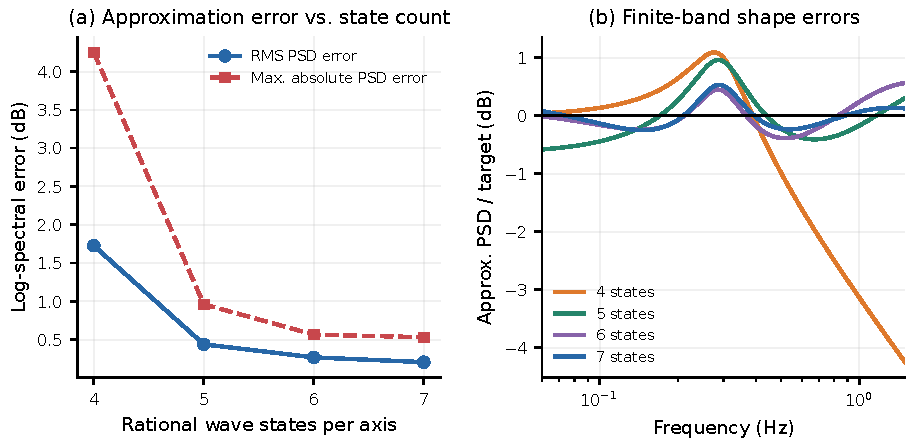
\includegraphics[width=.99\textwidth]{fractional-fig-5-rational-order.pdf}
\caption{Finite-band rational approximation of the
\(\nu=1.85,f_0=0.29\) Hz, \(\zeta=0.22\) transfer.
Real stable pole/zero ratios in (\ref{eq:frac-rat-family})
are fitted by deterministic complex-relative least squares on
0.06--1.50 Hz (five starting points per order, except order four).
Left: RMS and maximum log-PSD error versus \emph{wave states per
axis}; right: spectral residuals over the fitted band.
These are approximation errors, not measured CPU costs.
Fitted pole, zero, and gain values are saved in the JSON summary.}
\label{fig:frac-rational}
\end{figure*}

At 200 Hz the AtomS3R offers a nominal 5 ms interval, but whether
24--30-state nonlinear INS covariance prediction, measurement
updates, and parameter switching fit this budget must be determined
with the actual ESP32-S3 compiler and hardware. Dense matrix work
grows approximately quadratically/cubically with the implementation
structure; a state count alone cannot establish a CPU gain.
Finite-precision conditioning, memory, jitter, and periodic
covariance projections are part of feasibility, not afterthoughts.

\subsection{Three-Axis Spectral Structure and Multiple Seas}
\label{sec:frac-three-axis}
A direct XYZ extension uses three independent copies of
(\ref{eq:frac-hnu}), with 12--21 wave states after rational
approximation depending on order. That is simple, but
\(S_{p_i p_j}=0\) for \(i\ne j\) is usually not a
complete description of wave-induced orbital motion. A second
option keeps separate transfer functions but drives them with
correlated Gaussian innovations, so
\begin{equation}
S_{p_i p_j}(\omega)=
H_i(i\omega)Q_{ij}H_j(i\omega)^*.
\label{eq:frac-correlated}
\end{equation}
This supplies cross-coherence and phase structure only to the degree
that the restricted \(Q_{ij}\) and diagonal filters permit.
It does not amount to a directional hydrodynamic model.

A third option identifies a genuinely coupled multivariate state-space
spectral factor using (\ref{eq:frac-rao}), directional spreading,
encounter heading, and cross-axis phase relations. A fourth uses
shared latent swell and wind-wave sources, each driving several
motion axes through separate complex RAOs. Such sources can naturally
yield horizontal--vertical phase shifts and two distinct encounter
peaks. Independent CARMA priors in the existing XYZ benchmark do
not reproduce that full cross-spectral structure. Correlated
noise is a cheaper intermediate model; shared latent sources could
provide both greater physical coherence and a smaller state budget
than three separately duplicated high-order filters. Neither benefit
should be assumed without identification and replay.

Figure~\ref{fig:frac-mixed} tests the simpler scalar consequence
of spectral multimodality. The idealized incident spectrum is
a PM swell component (\(f_p=0.095\) Hz, \(H_s=1.25\) m)
plus JONSWAP wind waves (\(f_p=0.29\) Hz,
\(H_s=1.0\) m, \(\gamma=3.3\)).
To distinguish displacement from incident elevation, we explicitly
apply an \emph{illustrative, uncalibrated} heave response
\(|R(f)|^2=[1+(f/0.70\,\mathrm{Hz})^4]^{-1}\).
It is not a measured RAO or a claim about a particular hull.

\begin{figure*}[t]
\centering
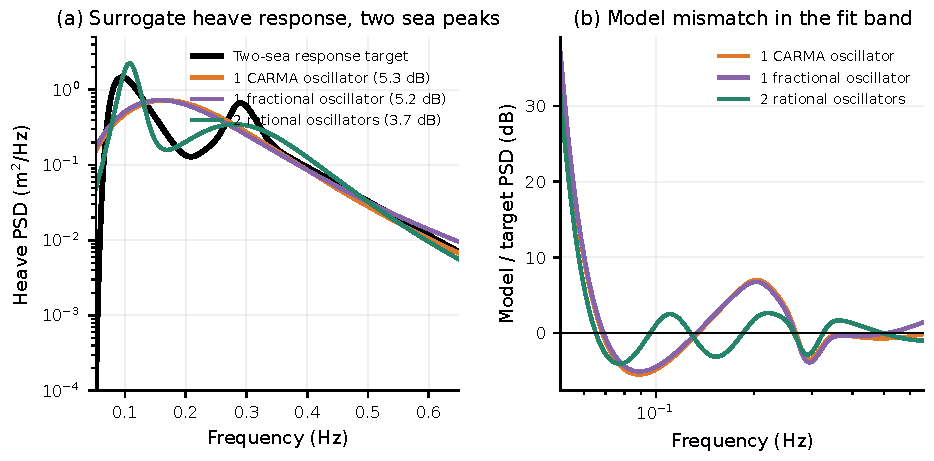
\includegraphics[width=.99\textwidth]{fractional-fig-6-mixed-sea.pdf}
\caption{Two-component, idealized \emph{surrogate vessel-heave} target:
PM swell at 0.095 Hz, JONSWAP wind waves at 0.29 Hz, and the
explicit illustrative RAO in the text. Compare a single
\(\nu=2\) repeated-oscillator CARMA(4,1), a single fractional
oscillator fitted over \(1.76\le\nu\le2.20\), and two
independent four-state rational oscillators whose PSDs add.
All models match total target response variance and minimize
(\ref{eq:frac-fit-objective}) over 0.051--0.66 Hz.
The two-component model uses eight wave states per axis if
naively replicated for XYZ. This is spectral-model evidence only.}
\label{fig:frac-mixed}
\end{figure*}

The weighted log-spectral errors are \(5.26\) dB for the single
integer oscillator, \(5.22\) dB for the single fractional
oscillator, and \(3.69\) dB for the two-component rational model.
The single fractional optimum reaches the allowed
\(\nu=1.76\) and \(\zeta=0.80\) bounds, indicating a constrained,
poorly identified compromise rather than a convincing gain.
The two-component advantage is specific to this controlled
two-peaked target and costs twice as many scalar wave states.
Equation~(\ref{eq:frac-peak}) explains why a single fractional
oscillator cannot reproduce two separated maxima. This suggests
testing physically meaningful component count and cross-axis
coupling before spending extra states only on fractional order.

\subsection{Falsifiable Ocean-IMU Experimental Roadmap}
\label{sec:frac-roadmap}
The next stage should use the \emph{same} three-axis CARMA benchmark
harness, independent truth generation, IMU forcing, initial states,
time stamps, calibration errors, and seeds for each candidate.
The comparison set must include: (1) unchanged shipping OU--III,
(2) experimental CARMA(4,1) XYZ, (3) CARMA(5,2) XYZ,
(4) a \(\nu\approx1.80\)--1.90 oscillator converted to a
stable rational order-5 or order-6 XYZ prior,
(5) tempered fractionally shaped CARMA(4,1), and
(6) two-component rational oscillators (possibly with
shared latent sources). Keep attitude, bias, magnetic,
startup, and time-step handling identical except where a
change is an explicitly declared experimental variable.

Truth conditions must include narrow and broad JONSWAP, PM,
long-period swell, mixed swell and wind, directionally spread
waves, multiple headings, stationary/still water, wave onset
and decay, accelerometer-bias uncertainty, and timestamp jitter.
Repeat with independent hull RAOs and withheld sea-state
parameters; do not score a model only on data drawn from its
own prior. Use matched seeds and paired uncertainty intervals
or a paired bootstrap to separate genuine changes from random
realization effects.

Report heave and horizontal displacement RMS and bias, maximum
startup displacement excursion, still-water phantom motion,
low-frequency and frequency-resolved error, attitude/translation
cross-contamination, NEES and NIS distributions with theoretical
confidence coverage, and divergence/negative-covariance counts.
For each variant also report total state dimension, model-switch
rate, process/measurement conditioning, 95th-percentile
AtomS3R execution time, and peak RAM/stack use at 200 Hz.
Process noise covariance, initial stationary covariance,
and each retune must be part of the tested specification.
An innovation sequence can appear white even when its
reported covariance is overconfident.

Existing complete-INS simulated CARMA evidence specifically warns
against accepting spectral fit alone. The
\texttt{docs/carma-three-axis.md} report records CARMA(5,2)'s
mixed-swell notch near \(0.09\) Hz and severe mixed-sea
accuracy loss, while CARMA(4,1) XYZ loses to OU--III in
mixed-sea heave. The same report documents on a still IMU
first-120-s heave startup RMS values of \(0.97\), \(2.96\),
and \(2.12\) m for OU--III, CARMA(4,1), and CARMA(5,2),
respectively (reported peak excursions up to \(2.5\), \(8.4\),
and \(6.0\) m). Six-dimensional mixed-sea NEES
was approximately \(31\), \(64\), and \(324\), respectively,
rather than the nominal dimension six. Those are
\emph{reported prior simulations, not fractional results}.
The extra poles and spectral tightness of a fractional approximation
could repeat or worsen both failures.

Proposed \emph{falsifiable}, pre-registered gates are:
\begin{enumerate}
\item A spectral candidate advances only if a held-out
\emph{vessel-displacement} cross-spectrum fit improves at
equal state count, without unacceptable near-DC energy or
acceleration regularity. A plausible early target is
\(E_{\rm dB}<1\) dB over an identified useful band, with
phase and integrated variance separately validated.
\item A full estimator advances only if paired heave and
horizontal RMS improve by at least 10\% on held-out
mixed/multimodal seas, with confidence intervals excluding
zero change. No quiet-water phantom, startup-peak, or
coverage metric may deteriorate materially relative to
OU--III; define precise per-case margins before testing.
\item Empirical 95\% covariance-coverage rates must lie
within their sampling-confidence intervals around the
nominal value, and NEES/NIS must not become more
overconfident. Stable float32 covariance, nonuniform
sampling, and live parameter changes must pass repeated
adversarial checks.
\item Peak measured update time must fit the complete
5 ms real-time deadline with a predetermined margin and
within measured AtomS3R memory. If extra states cause an
unacceptable cost, compare against a same-cost rational
model before attributing benefits to fractional calculus.
\end{enumerate}
Hypothesis F1: a constrained order-5 approximation of
\(\nu=1.85\) will preserve the fractional PSD to below
1 dB RMS over 0.06--1.50 Hz; Figure~\ref{fig:frac-rational}
supports this \emph{spectral} prediction only.
Hypothesis F2: this will improve paired INS RMS or covariance
consistency on held-out vessel histories; \emph{untested}.
Hypothesis F3: two physical wave components, or directional
cross-axis coupling, will outperform a single fractionally shaped
resonance on mixed seas at a controlled computational budget;
Figure~\ref{fig:frac-mixed} gives limited supporting spectral
evidence but no estimator evidence.
Each hypothesis fails if its stated gate fails; improvement in one
chart cannot override covariance or startup regressions.

\subsection{Prioritized Research Recommendation}
\label{sec:frac-recommendation}
\emph{First}, identify held-out, RAO-aware XYZ cross-spectra
for mixed swell and wind, and test shared wave components or
correlated excitation at a fixed state budget: this attacks a
documented CARMA failure and a physical structural omission.
\emph{Second}, test a tempered, fractionally shaped CARMA(4,1)
with enforced DC zero and acceleration regularity against
a same-order rational-only shaping baseline. The improved
fractional high-pass fits in Table~\ref{tab:frac-fair-refit}
motivate an additional \emph{state-budgeted} test, but a model
that merely reproduces their steep low-frequency cutoff using
eight or more states does not beat refitted five-state CARMA(5,2).
\emph{Third}, conditionally prototype an order-5
approximation to \(\nu\approx1.85\) in the \emph{benchmark},
only after independent vessel-response fits justify it and
the exact \(Q\), stationary covariance, and model-switching
tests pass. Fractional OU sea-state parameter dynamics are
a separate lower-priority experiment.

The present evidence establishes a mathematically coherent
fractional oscillator, a credible finite-band rational surrogate,
and a much better fit after adding a fractional high-pass factor.
An equally successful integer high-pass control and a better
cost- and objective-aware CARMA(5,2) refit show why spectral
flexibility alone does not prove a unique fractional advantage.
It does \emph{not} establish a fractional
three-axis motion prior superior in estimation accuracy,
stationary behavior, or runtime. Neither the stochastic-model
regularity calculation nor the existing shipping OU--III
stability proof transfers to a new estimator without a
new observability, covariance-consistency, model-mismatch,
and full-system stability analysis.
